\subsection{نگه داری سیستم (Maintain)}

با همکاری تیم های توسعه، عملیات، DevOps و مدیریت پروژه بر روی محیط Production لانچ می‌شود.
پس از آن عده ای از کادر فنی مسئول نگه داری از این سرور ها و برسی وضعیت سیستم خواهند بود.

البته این فقط بخش فنی ماجرا است. کادر مدیریتی و منابع انسانی نیز باید پاسخگوی تیکت ها باشند. سیستم نیازمند اپراتور است و نباید بدون پشتیبانی رها شود.


\subsubsection{مانیتورینگ}

برای جلوگیری از انواع ریسک ها، سیستم پیاده شده تمام اعلان ها و مشکلات فنی و مدیریتی خود را در ابزار هایی مانند Grafana نمایش می‌دهد.
داده ها و اطلاعات لحظه ای را می‌توان چه از داشبرد های درون برنامه ای و چه از Grafana مشاهده کرد.
اما به هرحال این پلتفرم، مناسب هم تیم فنی و هم تیم مدیریتی و محصول خواهد بود.

نمونه از تحلیل و داده های جمع آوری شده و نمایش آن بواسطه Grafana را می‌توانید ببینید.

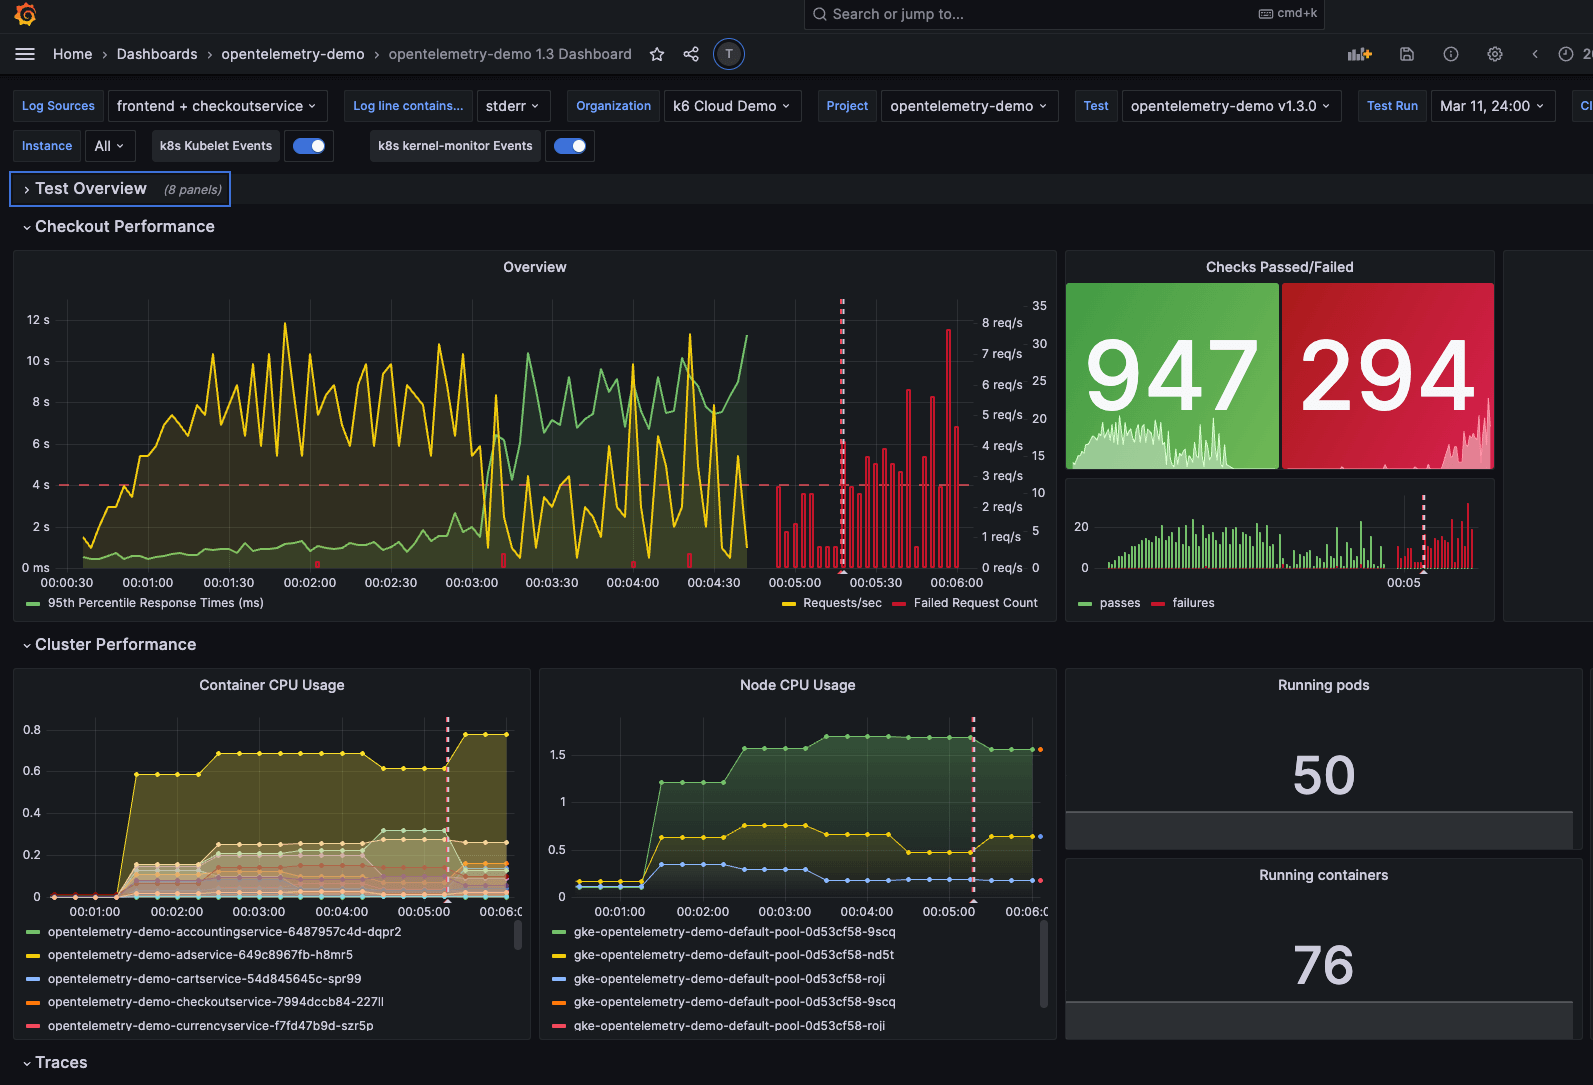
\includegraphics[scale=0.3]{assets/grafana.png}
